\documentclass[12pt]{article}
\usepackage{setspace, graphicx, fullpage, amssymb, amsmath, epsfig, natbib, array, multirow, hyperref}
\usepackage{amsfonts, bm} 
\usepackage{dcolumn}
\usepackage{subfigure, float} 
\usepackage[margin=.5in]{geometry} 
\usepackage{verbatim}
\usepackage{url}
\usepackage{enumerate}
\newcolumntype{d}[1]{D{.}{.}{#1}} 

\begin{document}
	
	\begin{center}
		Update: 07 December 2016, cont.
	\end{center}

This morning I have four additional replication tables for consideration. The first two are for the ``hybrid'' model (simulated annealing for 60 iterations and reassignment of ``flip flop'' votes after 30 iterations). The second is what we see from the ``flip flop'' reassignment algorithm with the stopping rule set to 150 iterations for all Congresses, as we were running it before. The final is an aggregate model of the effects of party calls in all Congresses using the ``flip flop'' reassignment model.

$ $

The hybrid model turns out similarly to the model that reassigns ``flip flop'' votes but doesn't use simulated annealing. We further find that forcing the ``flip flop'' reassignment algorithm to run 150 iterations rather than allowing it to stop after 15 iterations of less than 1\% of votes switching produces the same replication problem that we found before.

$ $

Given the short notice of this additional update, I will also bring this up in the meeting in case one or both of you understandably did not have a chance to look at this. Given what we find running the replication of tables and figures, we may have a problem in both these models in sorting votes with both these methods. Alternatively, I recognize that the general findings of the 2013 paper hold in the ``flip flop'' reassignment model if we take the results at the aggregate level we find what we expect to find with the responsive extremists hypothesis. The non-results of Congress 107 for Democrats are an oddity, but I am not familiar enough with this type of research to know how fatal they are to our replication findings.
	

\begin{table}
	\begin{center}
		\begin{tabular}{l c c c c c c }
			\hline
			& Dems 97 & Dems 102 & Dems 107 & Reps 97 & Reps 102 & Reps 107 \\
			\hline
			Ideological Extremism & $1.49^{***}$  & $12.76^{***}$ & $-1.39$        & $8.87^{***}$   & $7.35^{***}$   & $19.52^{***}$  \\
			& $(0.42)$      & $(2.16)$      & $(1.40)$       & $(0.62)$       & $(1.17)$       & $(2.36)$       \\
			Baseline rate of Voting with Party    & $1.02^{***}$  & $1.05^{***}$  & $1.29^{***}$   & $0.60^{***}$   & $1.12^{***}$   & $0.74^{***}$   \\
			& $(0.05)$      & $(0.12)$      & $(0.08)$       & $(0.05)$       & $(0.09)$       & $(0.09)$       \\
			Presidential Vote Share                  & $0.11^{**}$   & $0.11^{*}$    & $0.27^{***}$   & $-0.05$        & $-0.11$        & $-0.25^{***}$  \\
			& $(0.04)$      & $(0.05)$      & $(0.05)$       & $(0.05)$       & $(0.07)$       & $(0.05)$       \\
			South                     & $-4.26^{***}$ & $-3.84^{***}$ & $-0.16$        & $-1.49$        & $3.10^{**}$    & $0.94$         \\
			& $(0.84)$      & $(0.85)$      & $(1.11)$       & $(0.91)$       & $(1.01)$       & $(0.77)$       \\
			Vote Share                   & $-0.04$       & $-0.05$       & $-0.13^{**}$   & $0.07^{*}$     & $-0.01$        & $-0.03$        \\
			& $(0.03)$      & $(0.03)$      & $(0.04)$       & $(0.04)$       & $(0.03)$       & $(0.04)$       \\
			Female                    & $-0.71$       & $0.19$        & $2.34^{*}$     & $-2.41$        & $-0.39$        & $-1.09$        \\
			& $(1.81)$      & $(1.32)$      & $(1.07)$       & $(1.56)$       & $(1.85)$       & $(1.20)$       \\
			African American                      & $1.84$        & $-3.11$       & $-1.66$        &                & $-0.72$        & $-1.07$        \\
			& $(1.83)$      & $(1.70)$      & $(1.51)$       &                & $(5.01)$       & $(5.28)$       \\
			Latino                    & $2.46$        & $2.45$        & $-1.17$        & $2.78$         & $-5.80$        & $1.28$         \\
			& $(2.56)$      & $(2.05)$      & $(1.62)$       & $(4.44)$       & $(5.22)$       & $(2.14)$       \\
			Seniority                 & $-0.07$       & $0.15$        & $0.10$         & $0.12$         & $0.24$         & $-0.15$        \\
			& $(0.11)$      & $(0.11)$      & $(0.11)$       & $(0.13)$       & $(0.13)$       & $(0.12)$       \\
			Freshman                  & $-0.70$       & $0.49$        & $-1.82$        & $3.91^{***}$   & $1.79$         & $-1.91$        \\
			& $(1.27)$      & $(1.29)$      & $(1.75)$       & $(1.03)$       & $(1.50)$       & $(1.15)$       \\
			Retiree                     & $0.11$        & $0.34$        & $-2.00$        & $1.15$         & $-0.36$        & $-2.73$        \\
			& $(1.45)$      & $(1.00)$      & $(2.21)$       & $(1.46)$       & $(0.99)$       & $(1.57)$       \\
			Best Committee               & $0.09$        & $0.10$        & $0.17$         & $0.09$         & $-0.06$        & $0.26^{**}$    \\
			& $(0.08)$      & $(0.09)$      & $(0.09)$       & $(0.07)$       & $(0.10)$       & $(0.09)$       \\
			Party Leader                    & $3.64$        & $-1.02$       & $1.87$         & $0.79$         & $-0.87$        & $0.14$         \\
			& $(2.53)$      & $(2.16)$      & $(2.12)$       & $(1.88)$       & $(1.87)$       & $(1.79)$       \\
			Power Committee                     & $1.74$        & $1.36$        & $-0.21$        & $-3.15^{**}$   & $0.18$         & $-2.24^{*}$    \\
			& $(0.95)$      & $(0.99)$      & $(1.17)$       & $(1.05)$       & $(1.19)$       & $(0.91)$       \\
			Committee Chair                     & $2.38$        & $0.86$        & $-0.12$        &                & $0.48$         & $0.95$         \\
			& $(1.34)$      & $(1.47)$      & $(6.06)$       &                & $(4.94)$       & $(1.31)$       \\
			(Intercept)                 & $-5.10$       & $37.14$       & $-45.51^{***}$ & $-26.24^{***}$ & $-56.05^{***}$ & $-84.45^{***}$ \\
						& $(5.44)$      & $(20.52)$     & $(10.57)$      & $(7.24)$       & $(11.51)$      & $(15.32)$      \\
			\hline
			R$^2$                       & 0.82          & 0.79          & 0.74           & 0.75           & 0.76           & 0.68           \\
			Adj. R$^2$                  & 0.81          & 0.77          & 0.72           & 0.73           & 0.74           & 0.66           \\
			Num. obs.                   & 229           & 261           & 207            & 185            & 159            & 211            \\
			RMSE                        & 4.78          & 5.33          & 5.56           & 4.34           & 4.79           & 4.62           \\
			\hline
			\multicolumn{7}{l}{\scriptsize{$^{***}p<0.001$, $^{**}p<0.01$, $^*p<0.05$}}
		\end{tabular}
		\caption{House Replication ``Hybrid'' Model}
		\label{table:hybrid coefficients}
	\end{center}
\end{table}

\begin{figure}[h]
	\caption{Figure 2 Hybrid Model}
	\centering
	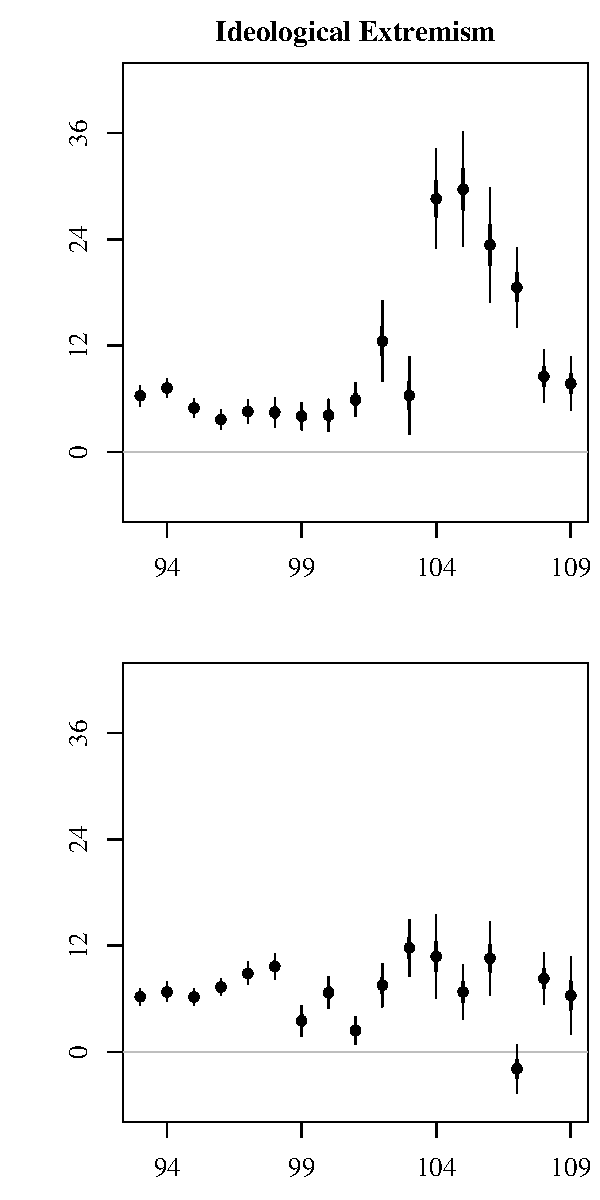
\includegraphics[width=\textwidth]{C:/Users/Ethan/Documents/GitHub/partycalls/plots/who-heeds-figure2-replication_hybrid.pdf}
	
\end{figure}

\begin{table}
	\begin{center}
		\begin{tabular}{l c c }
			\hline
			& Democrats & Republicans \\
			\hline
			Ideological Extremism & $3.26^{***}$  & $6.06^{***}$  \\
			& $(0.19)$      & $(0.23)$      \\
			Baseline rate of Voting with Party              & $0.97^{***}$  & $0.69^{***}$  \\
			& $(0.02)$      & $(0.01)$      \\
			Presidential Vote Share                  & $0.02^{*}$    & $-0.27^{***}$ \\
			& $(0.01)$      & $(0.01)$      \\
			South                     & $-4.31^{***}$ & $1.83^{***}$  \\
			& $(0.24)$      & $(0.27)$      \\
			Vote Share                   & $0.03^{***}$  & $-0.02$       \\
			& $(0.01)$      & $(0.01)$      \\
			Female                    & $0.62$        & $-1.89^{***}$ \\
			& $(0.35)$      & $(0.47)$      \\
			African American                      & $0.63$        & $-2.19$       \\
			& $(0.41)$      & $(2.43)$      \\
			Latino                    & $-0.50$       & $0.84$        \\
			& $(0.51)$      & $(0.98)$      \\
			Seniority                 & $-0.09^{**}$  & $-0.12^{**}$  \\
			& $(0.03)$      & $(0.04)$      \\
			Freshman                  & $0.71^{*}$    & $0.66$        \\
			& $(0.33)$      & $(0.37)$      \\
			Retiree                     & $-0.84$       & $-0.49$       \\
			& $(0.45)$      & $(0.49)$      \\
			Best Committee               & $0.07^{**}$   & $0.10^{***}$  \\
			& $(0.02)$      & $(0.03)$      \\
			Party Leader                    & $0.65$        & $1.70^{**}$   \\
			& $(0.60)$      & $(0.61)$      \\
			Power Committee                     & $1.21^{***}$  & $-0.22$       \\
			& $(0.29)$      & $(0.34)$      \\
			Committee Chair                     & $3.17^{***}$  & $2.20^{***}$  \\
			& $(0.46)$      & $(0.65)$      \\
			(Intercept)                 & $8.39^{***}$  & $-1.14$       \\
			& $(2.03)$      & $(1.95)$      \\
			\hline
			R$^2$                       & 0.73          & 0.62          \\
			Adj. R$^2$                  & 0.73          & 0.61          \\
			Num. obs.                   & 3982          & 3140          \\
			RMSE                        & 6.14          & 6.37          \\
			\hline
			\multicolumn{3}{l}{\scriptsize{$^{***}p<0.001$, $^{**}p<0.01$, $^*p<0.05$}}
		\end{tabular}
		\caption{Aggregate House Replication Hybrid Model}
		\label{table:coefficients}
	\end{center}
\end{table}
	
\begin{table}
	\begin{center}
		\begin{tabular}{l c c c c c c }
			\hline
			& Dems 97 & Dems 102 & Dems 107 & Reps 97 & Reps 102 & Reps 107 \\
			\hline
			Ideological Extremism & $1.39^{***}$  & $11.77^{***}$ & $-1.39$        & $8.65^{***}$   & $7.42^{***}$   & $21.06^{***}$  \\
			& $(0.41)$      & $(2.18)$      & $(1.48)$       & $(0.62)$       & $(1.22)$       & $(2.74)$       \\
			Baseline rate of Voting with Party              & $1.02^{***}$  & $1.12^{***}$  & $1.22^{***}$   & $0.60^{***}$   & $1.08^{***}$   & $0.59^{***}$   \\
			& $(0.05)$      & $(0.13)$      & $(0.08)$       & $(0.05)$       & $(0.09)$       & $(0.10)$       \\
			Presidential Vote Share                   & $0.10^{*}$    & $0.14^{**}$   & $0.29^{***}$   & $-0.05$        & $-0.15^{*}$    & $-0.28^{***}$  \\
			& $(0.04)$      & $(0.05)$      & $(0.05)$       & $(0.05)$       & $(0.07)$       & $(0.06)$       \\
			South                     & $-3.90^{***}$ & $-4.00^{***}$ & $-0.26$        & $-1.65$        & $3.27^{**}$    & $1.22$         \\
			& $(0.82)$      & $(0.87)$      & $(1.14)$       & $(0.91)$       & $(1.05)$       & $(0.83)$       \\
			Vote Share                  & $-0.04$       & $-0.06^{*}$   & $-0.14^{**}$   & $0.07^{*}$     & $-0.01$        & $-0.04$        \\
			& $(0.03)$      & $(0.03)$      & $(0.04)$       & $(0.04)$       & $(0.03)$       & $(0.04)$       \\
			Female               & $-0.63$       & $0.19$        & $2.56^{*}$     & $-2.35$        & $-1.73$        & $-1.46$        \\
			& $(1.77)$      & $(1.36)$      & $(1.10)$       & $(1.55)$       & $(1.92)$       & $(1.29)$       \\
			African American        & $1.55$        & $-3.22$       & $-1.88$        &                & $-2.09$        & $-2.16$        \\
			& $(1.79)$      & $(1.75)$      & $(1.55)$       &                & $(5.21)$       & $(5.70)$       \\
			Latino          &   $2.40$        & $2.45$        & $-1.40$        & $2.83$         & $-4.78$        & $1.13$         \\
			& $(2.51)$      & $(2.12)$      & $(1.66)$       & $(4.41)$       & $(5.42)$       & $(2.31)$       \\
			Seniority      & $-0.08$       & $0.13$        & $0.06$         & $0.13$         & $0.28^{*}$     & $-0.21$        \\
			& $(0.11)$      & $(0.11)$      & $(0.12)$       & $(0.13)$       & $(0.14)$       & $(0.13)$       \\
			Freshman         & $-0.67$       & $0.24$        & $-2.09$        & $4.08^{***}$   & $1.86$         & $-2.18$        \\
			& $(1.24)$      & $(1.33)$      & $(1.80)$       & $(1.03)$       & $(1.56)$       & $(1.24)$       \\
			Retiree           & $0.03$        & $0.20$        & $-2.05$        & $1.27$         & $-0.48$        & $-3.06$        \\
			& $(1.42)$      & $(1.03)$      & $(2.27)$       & $(1.45)$       & $(1.03)$       & $(1.69)$       \\
			Best Committee      & $0.09$        & $0.11$        & $0.19^{*}$     & $0.09$         & $-0.07$        & $0.30^{**}$    \\
			& $(0.08)$      & $(0.09)$      & $(0.09)$       & $(0.07)$       & $(0.11)$       & $(0.10)$       \\
		    Party Leader      & $3.51$        & $-0.80$       & $1.86$         & $0.92$         & $-1.44$        & $0.25$         \\
		    & $(2.49)$      & $(2.22)$      & $(2.17)$       & $(1.87)$       & $(1.95)$       & $(1.94)$       \\
			Power Committee       & $1.77$        & $1.27$        & $-0.39$        & $-3.06^{**}$   & $0.10$         & $-2.68^{**}$   \\
			& $(0.94)$      & $(1.02)$      & $(1.20)$       & $(1.04)$       & $(1.23)$       & $(0.99)$       \\
			Committee Chair      & $2.52$        & $0.85$        & $-0.08$        &                & $1.18$         & $1.41$         \\
			& $(1.31)$      & $(1.52)$      & $(6.21)$       &                & $(5.13)$       & $(1.41)$       \\
			(Intercept)     & $-5.10$       & $26.62$       & $-39.51^{***}$ & $-25.34^{***}$ & $-51.80^{***}$ & $-78.43^{***}$ \\
			& $(5.34)$      & $(20.84)$     & $(11.35)$      & $(7.19)$       & $(11.77)$      & $(17.34)$      \\
						
			\hline
			R$^2$                       & 0.82          & 0.77          & 0.71           & 0.75           & 0.75           & 0.66           \\
			Adj. R$^2$                  & 0.81          & 0.76          & 0.69           & 0.73           & 0.73           & 0.63           \\
			Num. obs.                   & 229           & 261           & 207            & 185            & 159            & 211            \\
			RMSE                        & 4.69          & 5.50          & 5.70           & 4.32           & 4.98           & 4.90           \\
			\hline
			\multicolumn{7}{l}{\scriptsize{$^{***}p<0.001$, $^{**}p<0.01$, $^*p<0.05$}}
		\end{tabular}
		\caption{House Replication Reassign Flip Flop Votes, forced to go 150 iterations}
		\label{table:house coefficients}
	\end{center}
\end{table}
	
\begin{table}
	\begin{center}
		\begin{tabular}{l c c }
			\hline
			& Democrats & Republicans \\
			\hline
			Ideological Extremism & $2.91^{***}$  & $5.84^{***}$  \\
			& $(0.18)$      & $(0.23)$      \\
			Baseline rate of Voting with Party              & $0.99^{***}$  & $0.70^{***}$  \\
			& $(0.02)$      & $(0.01)$      \\
			Presidential Vote Share                  & $0.04^{***}$  & $-0.26^{***}$ \\
			& $(0.01)$      & $(0.02)$      \\
			South                     & $-4.02^{***}$ & $1.85^{***}$  \\
			& $(0.24)$      & $(0.28)$      \\
			Vote Share                   & $0.03^{***}$  & $-0.00$       \\
			& $(0.01)$      & $(0.01)$      \\
			Female                    & $0.64$        & $-1.93^{***}$ \\
			& $(0.34)$      & $(0.48)$      \\
			African American                      & $0.47$        & $-2.32$       \\
			& $(0.40)$      & $(2.45)$      \\
			Latino                    & $-0.69$       & $0.66$        \\
			& $(0.49)$      & $(0.98)$      \\
			Seniority                 & $-0.10^{***}$ & $-0.12^{**}$  \\
			& $(0.03)$      & $(0.04)$      \\
			Freshman                  & $0.55$        & $0.87^{*}$    \\
			& $(0.32)$      & $(0.37)$      \\
			Retiree                     & $-0.86^{*}$   & $-0.50$       \\
			& $(0.43)$      & $(0.50)$      \\
			Best Committee               & $0.07^{**}$   & $0.11^{***}$  \\
			& $(0.02)$      & $(0.03)$      \\
			Party Leader                    & $0.59$        & $1.58^{*}$    \\
			& $(0.58)$      & $(0.62)$      \\
			Power Committee                     & $1.13^{***}$  & $-0.34$       \\
			& $(0.28)$      & $(0.34)$      \\
			Committee Chair                     & $2.92^{***}$  & $2.33^{***}$  \\
			& $(0.44)$      & $(0.65)$      \\
			(Intercept)                 & $4.10^{*}$    & $-2.07$       \\
			& $(1.99)$      & $(2.00)$      \\
			\hline
			R$^2$                       & 0.74          & 0.61          \\
			Adj. R$^2$                  & 0.74          & 0.61          \\
			Num. obs.                   & 3982          & 3140          \\
			RMSE                        & 5.94          & 6.43          \\
			\hline
			\multicolumn{3}{l}{\scriptsize{$^{***}p<0.001$, $^{**}p<0.01$, $^*p<0.05$}}
		\end{tabular}
		\caption{Aggregate House Replication Reassign Flip Flop Votes}
		\label{table:coefficients}
	\end{center}
\end{table}
	
	
	
	
\end{document}